\subsection{Overview}


This section describes the methods and materials sources we use for question generation and the training\&evaluation of the EQA system. The primary method relies on using utilities provided by the habitat platform. The name ‘Habitat’ is derived from the notion of learning within and from an environment(\cite{habitat19iccv}). The utilities in the platform provide necessary arrangements for the EQA task, such as simulating and working in a 3D environment, insinuating a robot with a specific configuration, preparing data sets, and setting up models for training. Materials are mainly used for question generation. The materials consist of data sets that contain semantic annotations and other geometric information essential for generating trainable episodes for navigation and VQA. 

The two components providing utilities in the Habitat Platform are referred to as ‘Habitat-sim'\footnote{ The GitHub repo for Habitat simulator \url{https://github.com/facebookresearch/habitat-sim}}, and ‘Habitat-Lab'\footnote{ The GitHub repo for Habitat Lab \url{https://github.com/Al-arug/habitat-lab}}. Habitat Simulator is a 3D simulator with multiple functionalities, such as facilitating configurable sensors and robots in 3D environments. The habitat lab is a library that contains multiple tasks that can be performed in the environment. The lab provides different models and training setups. In the following sections, we describe the two components and their usage in this project. 


The material we use for question generation is extracted from EQA-MP3D and Matterport3D. The environments in MP3D contain semantic annotations necessary for generating questions and the general linguistic understanding of the space. In addition, the annotations come with geometric information about the entities in the house, such as coordinate locations. The geometric information is essential for understanding the space geometrically for navigation as well as for question making. For example, asking a question about a spatial relation between two objects requires knowing where they are located. The task dataset,  EQA-MP3D, provides data for navigational training and information about the objects in the questions. Following the Habitat Lab and Simulator description, we outline the relevant material in the two data sets and explain some of the concepts necessary for understanding the usability of the extracted data. 



\subsection{Habitat Simulator}


Habitat-sim simulates 3D environments assimilating real-world settings. The environments are based on constructing either synthetic or real-world based scenes. \cite{szot2021habitat} describes a simulator as a system of two parts, physics engine, and renderer. The physics engine generates physical phenomena such as gravity and the physical state of the environment throughout the simulation, and the renderer completes the physics engine’s work by outlining objects, colors, and borders. When constructing the scene, habitat-sim can do environment state manipulation by changing the layout of objects \cite{habitat19iccv}. We observe a change of object’s layout, for example, in the names of objects in Matterport3D extracted from habitat-sim and the ones found in the MP3D annotation files. 

Habitat-sim has efficient GPU usage and can simulate different environment data sets. The simulation is displayed on GPU devices, which usually would require big storage of GPU to display a simulation of houses. The simulation setups in (\cite{szot2021habitat}, \cite{habitat19iccv}) allows for smaller storage GPU’s to perform the simulation. The latter makes it possible for an unfamiliar user of 3D simulation to simulate on their machines with reasonable speed. For the data set part, the simulator is designed with generalization for simulating different 3D Detests. In addition to MP3D, it supports 3D simulating for the following 3D datasets: GIBSON \cite{xia2018gibson},Replica\cite{straub2019replica}.


Habitat simulator facilitates the employment of configurable sensors and agents. Configurations such as the location to spawn the agent and the type of sensors, and their position on the agent are the types of flexible settings given to the simulator to act upon. “Sensors” is a different name for referring to the CNN decoders where each decoder can be seen as a sensor of the following: 1) RGB reconstruction, 2) semantic segmentation, and 3) depth estimation. The latter sensors are used to obtain “object attributes (i.e., colors and textures), semantics (i.e., object categories), and environmental geometry (i.e., depth).”. The agent can be configured with or more of the mentioned sensors depending on the task. For navigation, the agent is configured with “depth” and “RGB” sensors. Depth sensor is essential for the agent’s capability to navigate. With a depth sensor, it could estimate distances and avoid colliding with obstacles. For VQA, the agent is configured to output only “RGB” images of 5 frames. 



\subsection{Habitat Lab}

Habitat lab can be described as an API that facilitates task training in connection with the 3D simulator. In addition to initiating the simulator, Habitat-lab provides trainers, neural models, and data loaders. The lab has a hierarchical structure that acts given different configurations. For example, the steps for training/evaluating a task would be to prepare the data, initiate models and trainer, then simulate 3D environments. The information about the required model and the data for each task, such as paths to data and the models to use, can be manually given/changed in a task’s configuration file.

In addition to facilitating the training of whole tasks, the lab can train models separately. Concerning EQA,  the CNN model, in particular, is trainable independent of the other components using the lab platform. 

Training and evaluating the navigation and VQA is possible on baseline models\footnote{Instructions for training and evaluating the baseline models in the API \url{https://github.com/facebookresearch/habitat-lab/tree/master/habitat_baselines/il}}.
The text-image attention model is trained in connection with the pre-trained CNN\footnote{ File containing the VQA trainer \url{https://github.com/facebookresearch/habitat-lab/blob/master/habitat_baselines/il/trainers/vqa_trainer.py}} \footnote{ File containing the VQA model \url{https://github.com/facebookresearch/habitat-lab/blob/master/habitat_baselines/il/models/models.py}}. For navigation, the platform provides a training setup for Imitation Learning. 

As mentioned earlier, for a VQA training and evaluation session, the lab facilitates preparing the VQA dataset in a conventional VQA format. Data preparation and setting up the models \& trainer acts upon the paths and settings given in the VQA configuration file \footnote{Configiration files for baseline including VQA config \url{https://github.com/facebook research/habitat-lab/tree/master/habitat\_baselines/config/eqa}}. The configuration file also includes some manually instructed commands for configuring the robot, where the lab passes these instructions to the simulator. The simulator is initiated simultaneously while preparing the VQA dataset. The data loader of the lab takes each environment ID from each QA sample in the EQA dataset and extracts the image frames. 

Besides facilitating EQA training, the lab contains training setups for other tasks. The trainable tasks in the platform are as the following
Goal navigation where the robot has to navigate to a geometric point;
object navigation where the system has to navigate to an object;
pick-up task where the robot has to pick up an object and move it to a different location, language-vision task where the agent follows directional instructions.
Each of the previously mentioned tasks has a separate data set. 



%Hence- current hidden-state h_{t} and the current action are the only %updated in the planner: 
%
%The controller executes the action a_{t+1}. It takes then the 
%
%Hence, h_{t-1} and a_{t-1} carry no information at the 0 timestep %since no encoding or action has been output by the planner at the 0 %step; Thus, they are more like an initiation in this example.  
%
%The planner passes the current action a_{t} and the currently hidden %state h_{t} to the controller 
%

\subsection{Data and Data-sets}

In this section, we review the materials used in generating QA episodes. The first part is a review of data structure and the relative semantic annotations found in MatterPort3D. The review of MP3D also includes an elaboration of geometric and viewpoints concepts necessary to understand the geometric annotations in MP3D and their usage. The second part of this section includes a review of the EQA-MP3D dataset structure and content.

EQA-MP3D is seen as a method and material source. The method of generating QA episodes relies on imitating EQA-MP3D. The imitation of EQA-MP3D ensures that the newly generated QA episodes are executable in the habitat platform by matching code requirements. Having the same structure for the generated question-answers as EQA-MP3D, a review on EQA-MP3D would also help imagine the QA form that this project achieves.   In the same review, the navigational data we take as a material source for navigational training are highlighted and explained. 

\subsubsection{Semantic annotations in Matterport}

%(restructuring is required-- more precision) (examples to rephrase-- why do we need the %location in global coordinates and why the camera views are also important)
\paragraph{Annotations}

In the Matter port annotations, each house environment has three files. The three files are x.house,x.ply, and x. We collect the annotations from the x.house files house. 

Each house file (x.house) has eleven line-types of annotations.\footnotetext{https://github.com/niessner/Matterport/blob/master/data\_organization.md}. The lines are marked by a capital letter as a marker; the first letter-marking to the last letter areas in this list [H, L, R, P, S, V, P, I, C, O, V]. Each letter-marker symbolizes a certain type of information. In this section, I will explain only the type of information that we use in this project.

The line representing an object’s info in a house file begins with the string “O”. The “O” lines contain information about the objects in the house. Every line that begins with an O letter consists of one object in the house with corresponding information about its geometry and location within a room and level floor. Each "O" line looks as such: [ O object\_index region\_index category\_index px py pz  a0x a0y a0z  a1x a1y a1z  r0 r1 r2 0 0 0 0 0 0 0 0 ] 

The object's data in the line seen above comes in a string form, and each section in the string represents different types of information. \textit{Object\_index}, the index of an object is what we refer to as the object ID. \textit{region index} is the room ID. \textit{category\_index} is the object’s index in the category map; this index is used to obtain the object’s name from the category map.\textit{px py pz} represent the center of the box in (x,y,z) axis. \textit{r0 r1 r2} represent the radius of the object from the center on the (x,y,z).\textit{a0x a0y a0z  a1x a1y a1z} these are the rotation of the OOBB radius(OOBB and radius will be elaborated on in a coming section). Finally, the last “0” s in the line have no meaningful value and therefore are ignored. 

\paragraph{Point of views,  geometric data}

As seen in the previous section, the geometric information consists of elements as the location of an object, region, or level, defined by their center in a world coordinate system. Other information is the size of the entity given its radius from its starting location (center).   

The camera views of the scenes are globally oriented \cite{Matterport3D}(p3). A way to allocate an object is to find its location under global coordinates. Let’s say the global coordinates start from the center of a house where the center of the house is (0,0,0) on the (x,y,z); and let’s say all the objects are spawned throughout the house’s (x,y,z) axis where its distance defines the location of each object to the house center. When annotated, the objects are viewed through a camera. The description of their geometric location, thus, should consider the view-position of the camera. 

\begin{figure}[H]
\centering
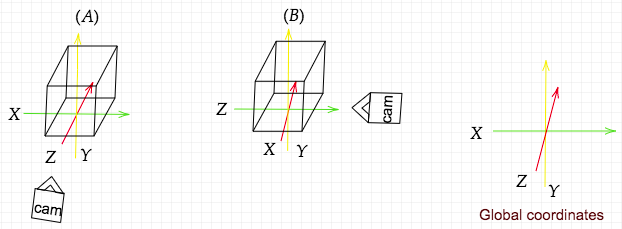
\includegraphics[scale=0.53]{images/campos.png}
\caption{The camera in graph A views the objects from global perspective(readers perspective). The view of the camera in graph B is rotated. The rotation is resembled in the the axis's representation }
\label{fig:campos}
\end{figure}

In graph (A) in \ref{fig:campos}, we see that the camera-view of coordinates aligns with the global coordinates. The (x,y,z) that go through each object in graph(A) and graph (B) are the view of the axis in reference to the camera. However, if the camera is positioned to the right of the object from our view, as in graph (B), then we say that the camera view of coordinates is not aligned with the global view. We notice in graph (B) that from the camera view, the “global X” is “Y” and vice versa.

Some geometric calculations cannot be performed if the location measurements are not relative to each other. For example, if we want to calculate the distance between objects, the locations must be consistent with one reference point. The camera position is changing, and if the camera’s position references the location of an object, we would get locations relative to the changing position of the camera in timespan. 

To globalize the view's orientation, measures such as top-down view of a map or calculating the camera's rotation from the global center. While the global locations are crucial for measuring the distance, other point-views are also crucial for other purposes. There are three essential coordinate systems to know when working in a 3D environment: 

\textbf{1. World coordinates}(global):  World coordinates(global): The coordinate system that starts at the center of the world; a house in our example. Its distance then decides the center of an object in this coordinate system to the center of the world. 

\textbf{camera-view coordinates:} The coordinates from the camera’s views. The center of this coordinate system is the position of the camera. Its distance to the camera defines the center of the object in this world. 

\textbf{3. Local view:} The center of the local view is the object itself. 

The center of all these views is (0,0,0). We described above that the world coordinate system allows us to measure the distance between objects in a world map. The camera view is useful if a robot is expected to navigate an environment and describe spatial relations between objects such as “next to”, “above”. The local view could tell about the size of an object. In particular, the (x,y,z) from a local point of view tell about how far the object stretches from its center where the center is (0,0,0). The local view can be referred to as “radius”. 

matterport 3D provides the views described above. Next, We discuss the usage of the object’s location in global coordinates and the local view in detail. 

\paragraph{Object's locations, geometric data}

\begin{figure}[H]
\centering
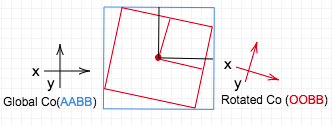
\includegraphics[scale=0.5]{images/A-OB.png}
\caption{2D AABB represented in blue square with its axis aligning with the world view of axis. 2D OOBB represented in red square has its axis rotated from the global view }
\label{fig:A-OB}
\end{figure}

In a 3D environment, objects could be represented by bounding boxes(covers) referred to as “Axis-Aligned Bounding Box” (AABB) and “Object-Oriented Bounding Box” (OOBB).

The AABB and its center are aligned with the view of the world coordinates, while the OOBB is oriented with the box and more likely to be rotated from the global view. In figure \ref{fig:A-OB} we see a demonstration of the two boxes in 2d squares. The red square represents the ‘Object-Oriented Bounding Box’ (OOBB), where its (x,y) radius connecting the center to the sides is colored in red. The blue square represents the ‘Axis Aligned Bounding box’ (AABB), where its (x,y) radius connecting the center to the sides is colored in blue. The notable difference between the two boxes is the direction of their radius. The radius of the AABB in black is aligned with the direction of the global coordinates on the right part in \ref{fig:A-OB}. The radius of OOBB, on the other hand, has its coordinate direction rotated from the global coordinates illustrated in the red coordinates on the right side of the graph. 

The difference in the rotation of the coordinates is important for determining the correct calculation for estimating the locations of the box’s sides. In order to obtain where the sides/corners of the box are located in the global coordinates, we would estimate how far the radius-es stretch from the center and in what direction.

The estimation for the AABB sides is straightforward since the AABB’s radius stretches in the same direction as the global coordinates. For example, subtracting the length of the AABB radius on the y-axis from the center would give us a location point of the lower horizontal line of the blue box. Adding the (y) length from the center point would give a location point on the upper side of the blue box. Hence- The center and the AABB radius are both globally aligned(pointing in the same direction) so adding or subtracting them would give the correct globally defined position of the AABB side.

Even though the centers of OOBB and AABB are positioned in the same location, the direction of their axis is different. For estimating the sides of the OOBB from the center, one should consider the rotation of the coordinates. Adding or subtracting the OOBB (x,y) radius from the center, as done for the AABB in the previous example, would likely not end in a correct position on any OOBB sides since the directions of the coordinates(slope) are different. Estimating a globally defined point on any OOBB sides would require calculating the rotation or the slop of the radius from the center (the direction). 

Using the AABB of an object is suitable for a direct allocation of the geometric locations of objects. At the same time, OOBB could give a more accurate estimation of the size of an object. With AABB, the borders of an object could be found with straightforward calculation, which makes it less complex. For example, allocating two objects and calculating the distance between any side would only require knowing their radius and centers. The OOBB, on the other hand, is more enclosed in the object since it’s more oriented in the object’s local view. The enclosing of the OOBB on the object makes the space between the box sides and the object's edges much smaller compared to the space that could be found in an object defined in an AABB. The radius of the OOBB can provide a more accurate measurement of the object’s volume. For size estimation, the rotation is unnecessary because calculating the volume does not require knowing any coordinate positions in a global map.  



\subsubsection{EQA (Task Dataset)}

Our method for generating questions relies on imitating the structure of the EQA-mp3d dataset. In this section, we give a review of the EQA-mp3d structure and content. The EQA-mp3d also provides a primary material source. The relevant material consists of the navigational data required for constructing a trainable episode. In addition, an episode includes essential information about the target object in a question, such as its ID and room ID. This object's info is important as it would make it possible to acess more metadata about the spcefic object from the annotation. 

\paragraph{Structure}

%\begin{figure}[H]
%\centering
%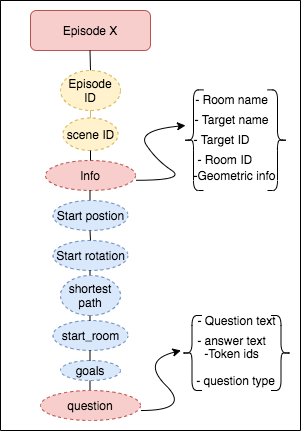
\includegraphics[scale=0.5]{images/episode1.png}
%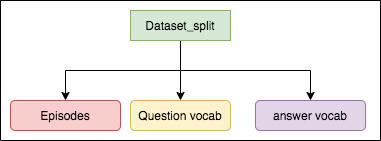
\includegraphics[scale=0.5]{images/datasplit1.png}
%\caption{}
%\label{fig:episode}
%\end{figure}

\begin{figure}[H]
    \centering
    \subfloat[]{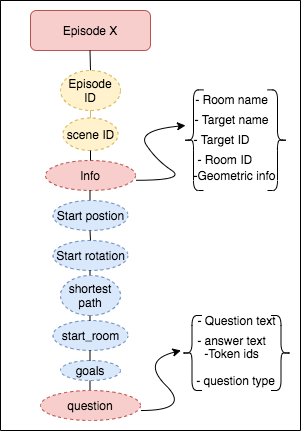
\includegraphics[scale=0.5]{images/episode1.png}}%
    %\qquad
    \subfloat[]{{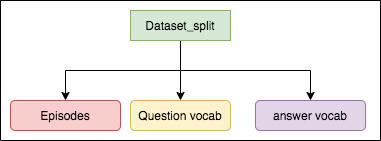
\includegraphics[scale=0.5]{images/datasplit1.png}}}%
    \caption{ (A) represents the structure of one QA episode. The arrow and curly brackets branching from "info" and "questions" show the content of each of these two categories. (B) represents the most top layer of a split("train" or "val")}
    \label{fig:episode}
\end{figure}.



Figure \ref{fig:episode} (B) shows the top structure of the val and test. \textit{Episodes} contains all QA episodes in a data-set split. \textit{Question vocab} and \textit{answer vocab} contain the same elements as dictionary keys. The elements are: [word list,stoi,itos,num vocab,pad token].

“Question vocab” and “answer vocab” in the “train” and “Val” are identical to each other. When using each split of the dataset, the answer-tokens that are considered are the ones contained within the episodes instead of the word lists mentioned above. 

Each question-answer is an episode that consists of multiple layer information. The structure of an episode is as seen in \ref{fig:episode} (A). We describe the elements of an episode in the following:  

\textbf{House ID}: The house ID given by the house ids in MatterPort3D.\\
\textbf{Episode ID}: The episode index in the range of the split’s length. \\
\textbf{Info}: This element contains all the information about the object and room in a question. The inner layers of “info” include the following: 

Information about the target object is the first layer within “info” and its elements are listed below: 

\textit{centroid}: The center of the object’s Axis-aligned bounding box(AABB). The center coordinates are in 3D on the (x,y,z) axis and defined with the global view. 

\textit{radi}: This is the radius of the Axis-Aligned-bounding box of the object. The AABB radius is in 3D on the (x,y,z) axis. 

\textit{level}: The level-floor number in the house where the object is located. 

\textit{room-id}, \textit{obj Id},\textit{room name}, \textit{object name name}: Room ID, room name and object ID as given by semantic annotation in  Matterport3D. Many of the objects are re-named, mostly names in hyponymes changed to hypernym category such as: round-sofa, l-shaped sofa changed to their hypernym category "sofa". The  information about the room (\textit{room-id},and \textit{room name})  are found in the second layer within "info"


The elements that are marked in blue in figure \ref{fig:episode} are \textbf{navigation data} used for training the navigator:

\textbf{Start position}: The start positions are all unique. For each unique question in the data set, there is fifteen different starting position. 

\textbf{Rotations}: These are the rotations that the agent has to do while navigating. It stands as supplementary information for the shortest path. 

\textbf{Shortest Path}: The shortest path is the data used for Imitation Learning by training the robot to follow the steps in the path with short rewards. The path consists of steps in frequencies that mark the shortest way to reach the question's object. 

\textbf{Goals}: Goals are the destinations that the agent should reach in navigation. The goals stand for the viewpoint where the robot can see the target object. Each viewpoint consists of a geometric position and the rotation toward the target object respective to the position. 




%\begin{figure}
%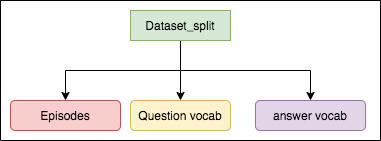
\includegraphics[scale=0.5]{images/datasplit1.png}
%\end{figure}







